\documentclass[12pt]{article}

\usepackage[MeX,T1,plmath]{polski}
\usepackage[utf8]{inputenc}
\usepackage{graphicx}
\usepackage{indentfirst}


\author{Michał Burdukiewicz}
\title{\large Wsparcie aktywności naukowej doktorantów, studentów i Studenckich 
Kół Naukowych- Wydział Biotechnologii, Uniwersytet Wrocławski 
\\ 
01.12.2015-15.12.2015 \\ 
\normalsize Sprawozdanie}

\date{}

\begin{document}

\maketitle

Dzięki środkom finansowym przyznanym przez Konsorcjum Wrocławskie Centrum 
Biotechnologii Doktoranckie Koło Naukowe Bioinformatyki  
zrealizowało projekt ``Predykcja białek amyloidogennych''.

W trakcie badań opracowano probabilistyczny model miejsc amyloidogennych za 
pomocą metod analizy języka naturalnego. Stworzony model nie tylko w 
intuicyjny sposób opisuje strukturę miejsc inicjacji agregacji, ale również 
pozwala przewidywać białka amyloidowe. Dokładność predykcji naszego programu 
jest dużo większa niż innych istniejących programów tego typu. Przeprowadzenie 
obliczeń, niezbędnych do realizacji tego zadania badawczego, nie byłoby 
możliwe, gdyby nie modernizacja istniejącej infrastruktury dzięki środkom 
finansowym przyznanym przez Konsorcjum.

W ramach projektu przygotowano następujące komunikaty konferencyjne w postaci 
posteru:
\begin{enumerate} 
\item Burdukiewicz M., Sobczyk P., Mackiewicz P., Kotulska M., 
\textit{AmyloGram: n-gram analysis and prediction of amyloids}, 
\textbf{Bioinformatics in Toruń}, 16-18 czerwiec 2016, Toruń (Polska) (zał. 1)

\item Burdukiewicz M., Sobczyk P., Rödiger S., Mackiewicz P., Kotulska M., 
\textit{AmyloGram:a novel predictor of amyloidogenicity}, 
\textbf{European Conference on Computational Biology}, 3-7 września 2016, 
Haga (Holandia) (zał. 2)
\end{enumerate}

Wyniki badań zostaną również przedstawione w postaci wystąpienia podczas 
kongresu \textbf{German Conference on Bioinformatics} (12-15 września) w 
Berlinie (Niemcy) (zał. 3) i opublikowane w \textbf{PeerJ Preprints}. 
Niezależnie trwa przygotowanie manuskryptu opisującego otrzymane 
rezultaty.

Prezentacja wyników na tak szeroką skalę nie byłaby możliwa, gdyby nie 
dofinansowanie wyjazdów zagranicznych przez Konsorcjum. Dzięki wsparciu 
finansowemu mamy możliwość przedyskutowania naszych rezultatów z wieloma 
naukowcami, co pozwoliło nam przeprowadzić znacznie ulepszyć stosowane metody 
badawcze.

\clearpage

\large{ZAŁĄCZNIK 1}

\begin{center}
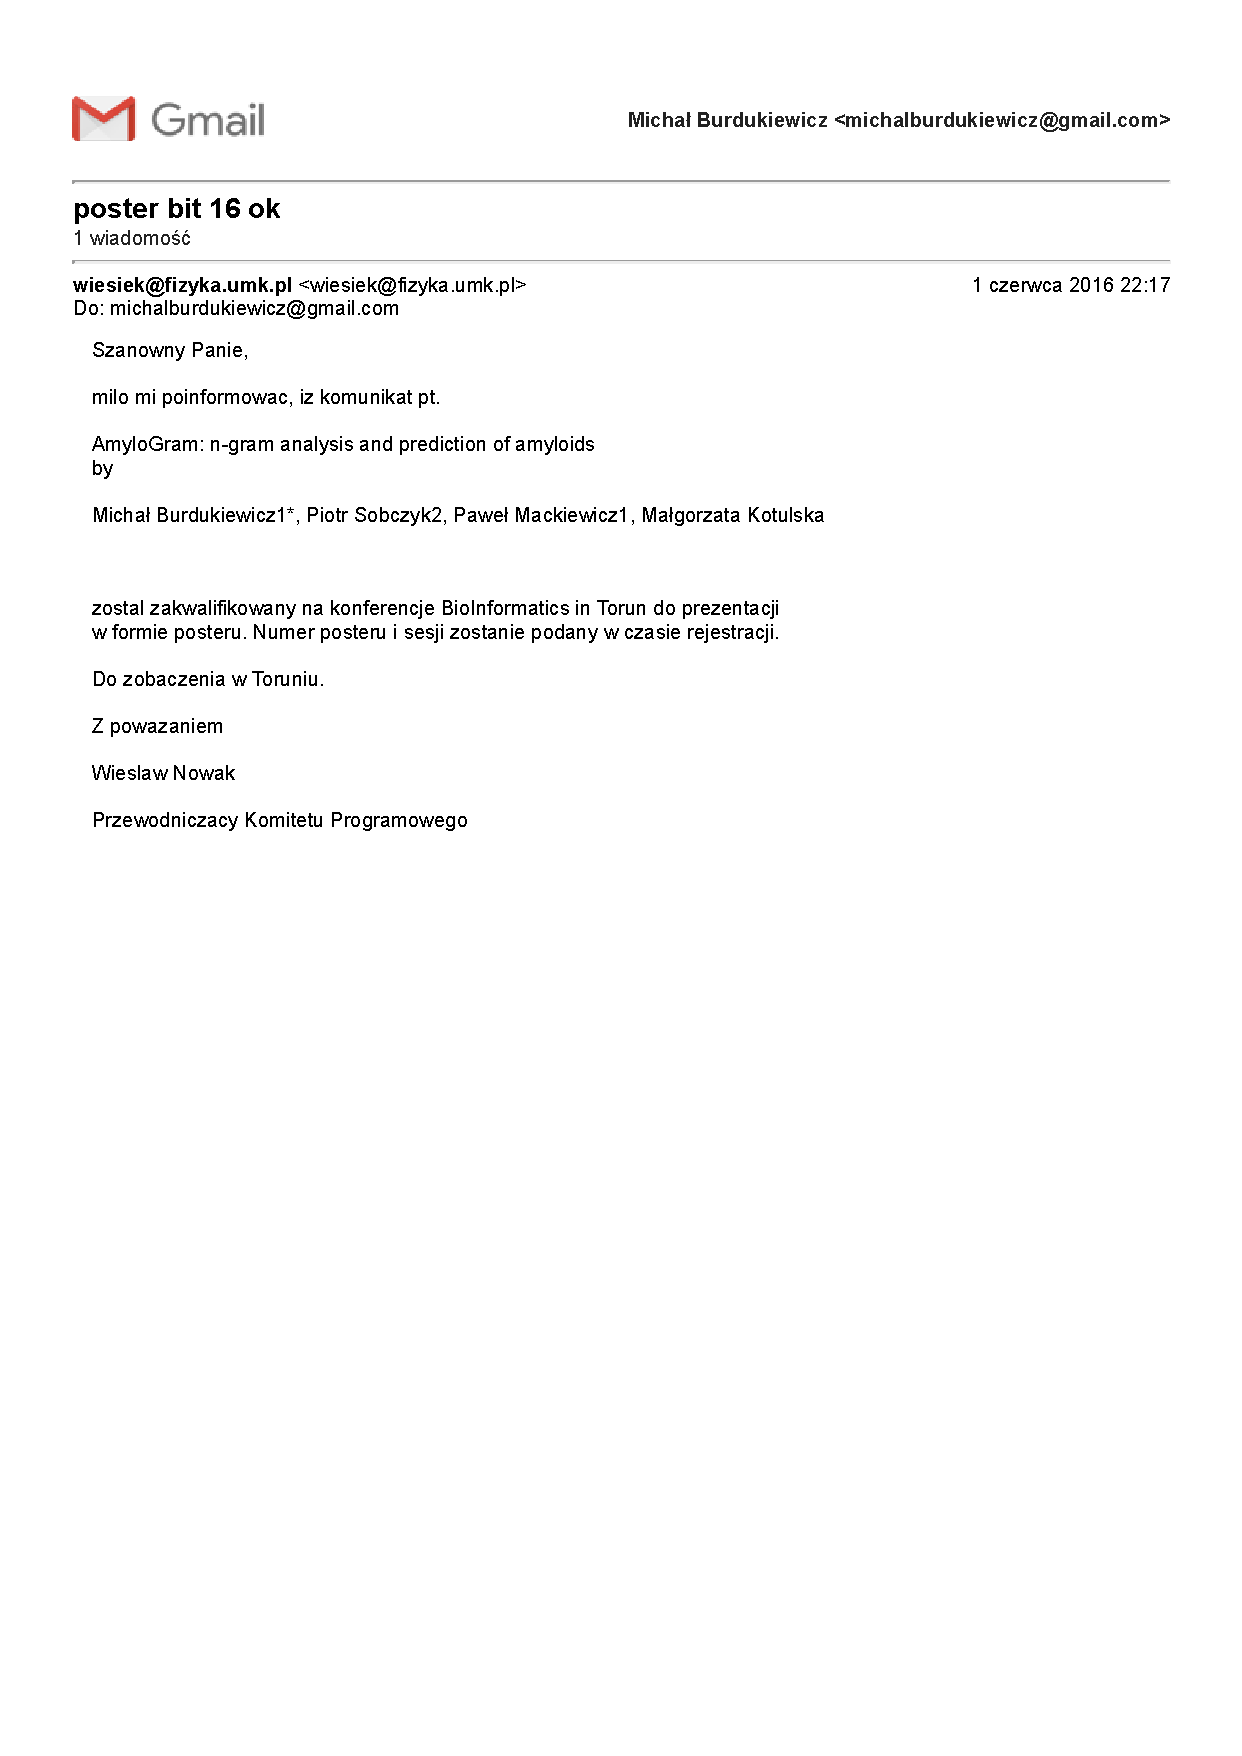
\includegraphics[width=0.95\linewidth]{amyloids/BIT2016.pdf}
\end{center}
\clearpage


\large{ZAŁĄCZNIK 2}

\begin{center}
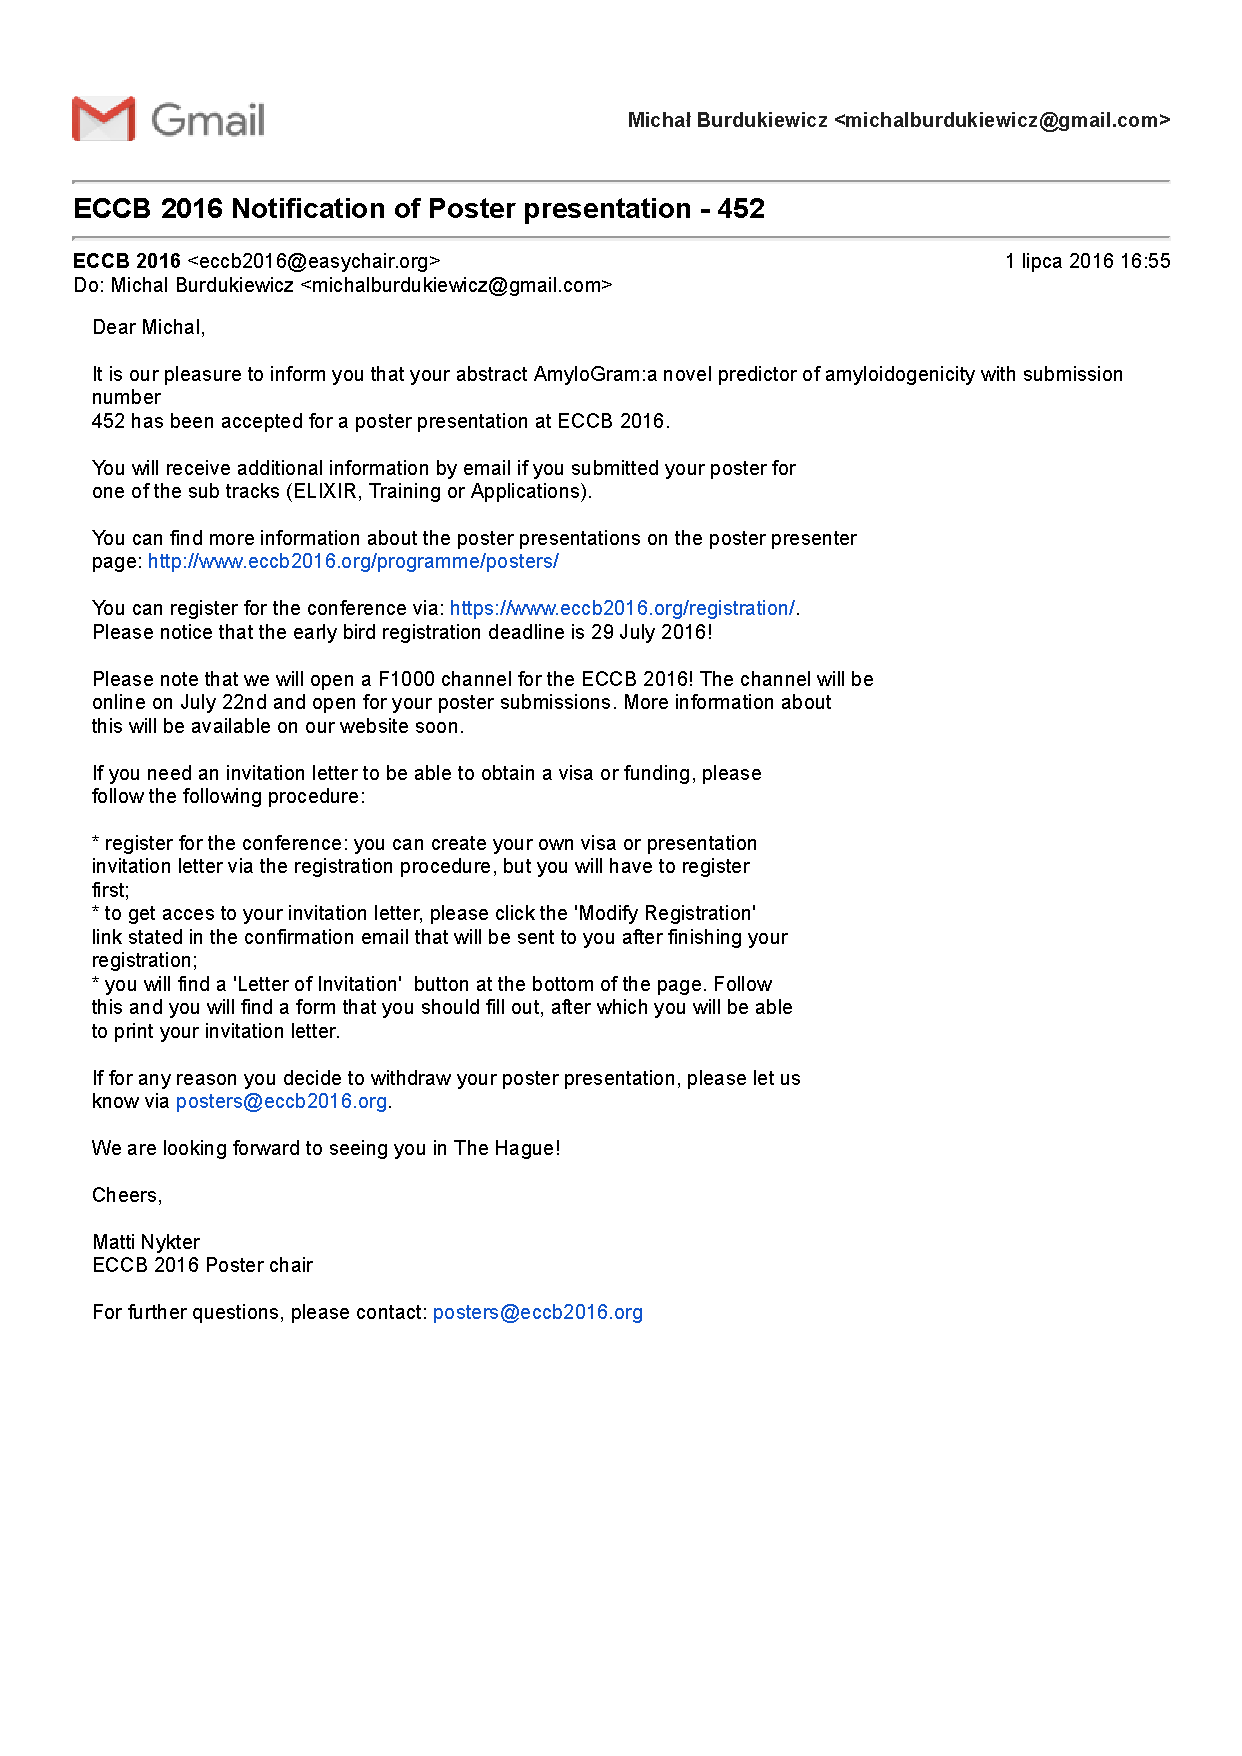
\includegraphics[width=0.95\linewidth]{amyloids/ECCB2016.pdf}
\end{center}
\clearpage

\large{ZAŁĄCZNIK 3}

\begin{center}
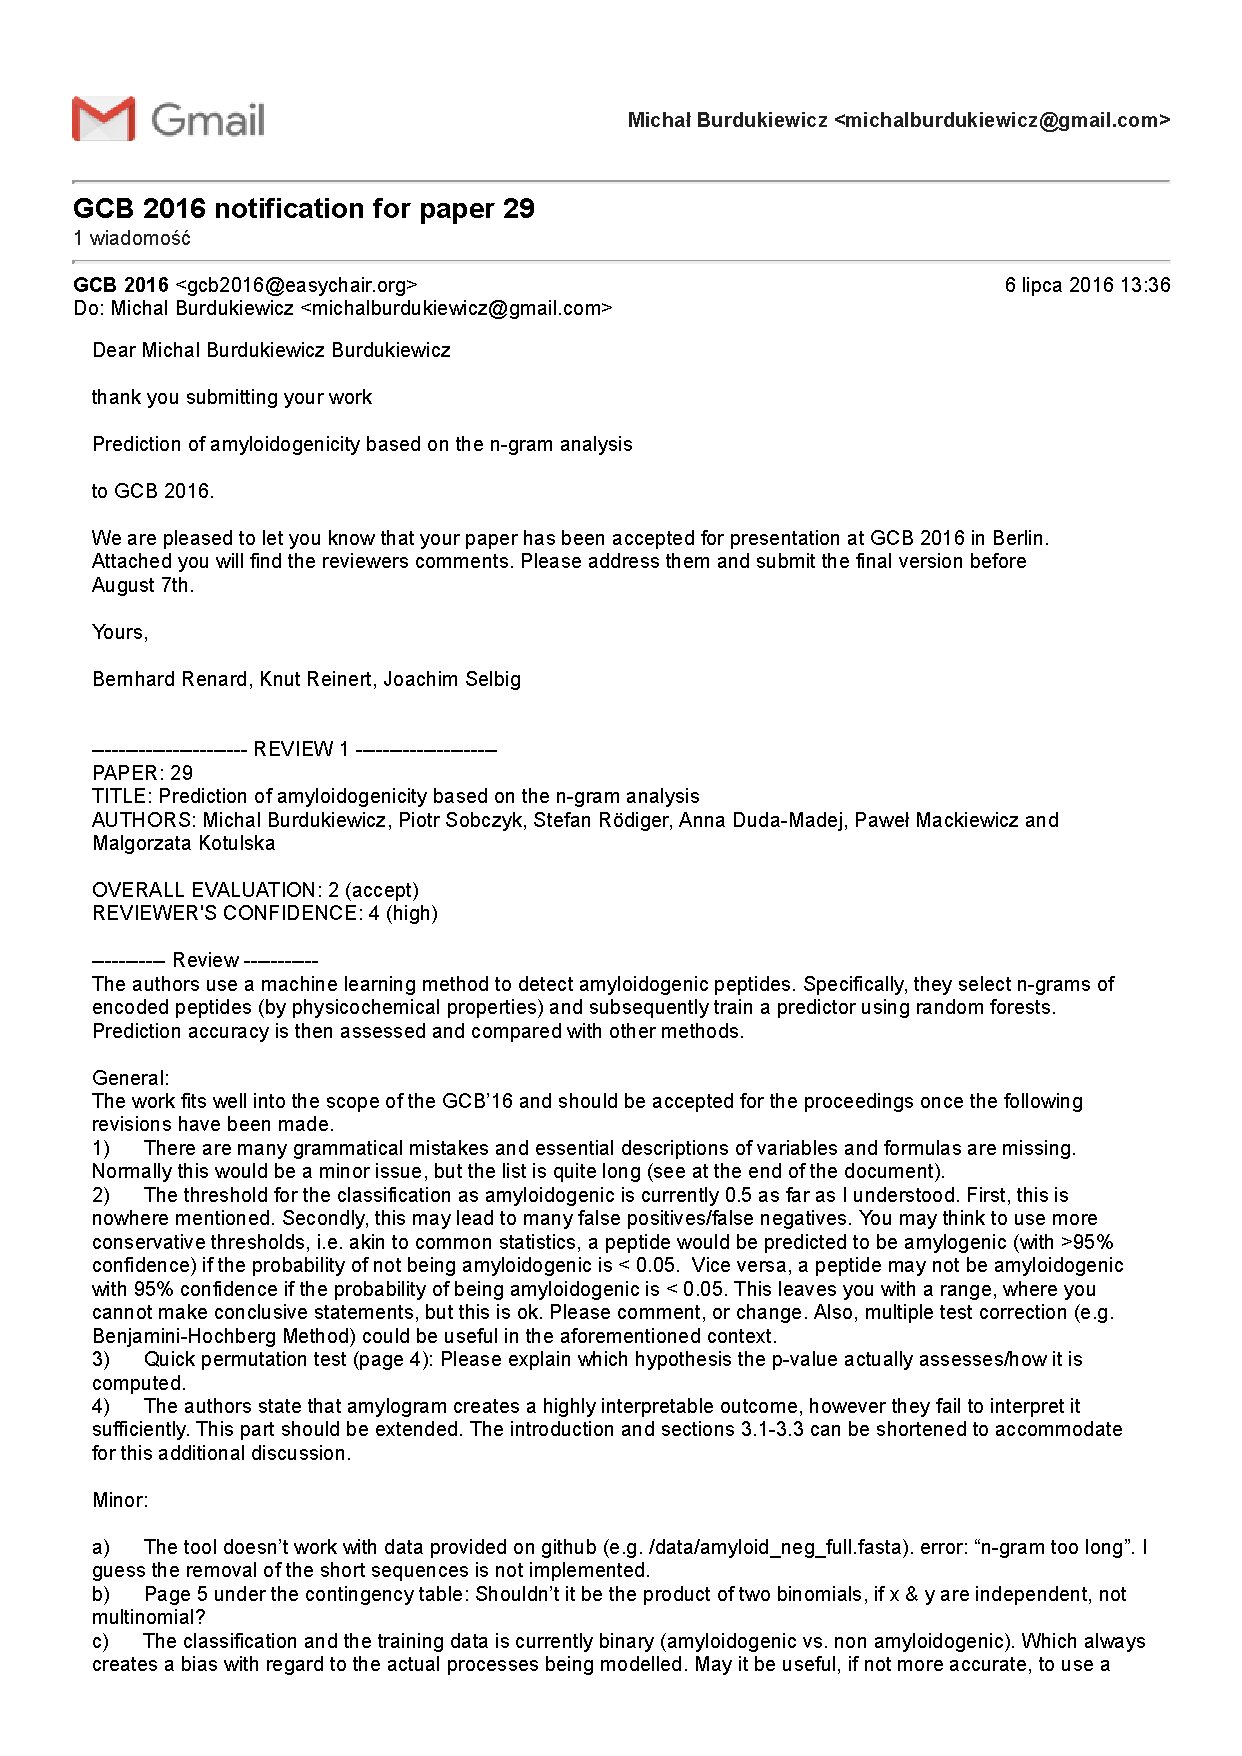
\includegraphics[width=0.95\linewidth]{amyloids/GCB2016.pdf}
\end{center}
\clearpage

\end{document}
